


Dans la littérature on observe de nombreuses œuvres de synthèse visant à caractériser et classifier les différents problèmes appartenant à la classe \wsrp.
Desrochers \cite{Desrochers1990} propose une classification des \wsrp qui étend celle des problèmes d'ordonnancements classiques $\alpha~|~\beta~|~\gamma$.
Desrosiers \cite{Desrosiers1995} montre l'évolution des problèmes de routage avec fenêtres temporelles et propose une méthode pour les résoudre.
L'étude menée par \cite{Solomon1988} sur les \wsrp vise à exhiber les avancées sur les différentes méthodes de résolutions pour les \wsrp.
Pillac \cite{pillac2012dynamic} définit les problèmes de routage dynamique stochastique ou déterministe et propose des algorithmes et heuristiques pour les résoudre.



Pour résoudre les problèmes appartenant à \wsrp, on observe dans la littérature de nombreuses méthodes comme les méthodes exactes (Constraint Programming ou Integer Programming), les méta-heuristiques (recuit simulé, recherche tabu, génétique, ...) ou encore les méthodes hybrides.

En pratique ce sont les méthodes hybrides qui sont utilisées, car elles s'adaptent plus facilement lorsque la taille des instances devient grande.

Pour les méthodes exactes on retrouve : pour les modèles en PLNE une résolution à base de génération de colonnes en utilisant une décomposition de Dantzig-Wolfe.
Le problème maître est un problème de partition (set partitioning en anglais) et le sous-problème est un problème de Plus Court Chemin avec Fenêtres Temporelles (Elementary Shortest Path Problem with Time Windows en anglais). Ensuite la génération de colonnes est mélé à un algorithme de branch-and-price afin d'améliorer la convergence. 
En général, en plus d'utiliser le modèle PLNE, on retrouve dans la littérature l'utilisation des méta-heuristiques pour obtenir une bonne solution initiale afin d'obtenir de bonnes bornes entières.

\wsrp combine la complexité des problèmes d'ordonnancement \cite{Blazewicz1983,Lageweg1982} :
\begin{itemize}
\item ordonnancement de projet à compétences multiples (Multi-skill Project Scheduling Problem, Tehcnician and Task Scheduling Problem).
\item Séquençage et ordonnancement de tâches (Sequencing and Scheduling Problem) \cite{Lawler1993}.
\item Ordonnancement de projet avec contraintes de ressources (Resources Constrained Project Scheduling Problem).
\end{itemize}
et des problèmes de tournée de véhicule \cite{Lenstra2013,Tsitsiklis1992} :
\begin{itemize}
\item Problème de tournée de véhicules avec fenêtre de temps (Vehicule Routing Problem with Time Windows).
\item  problème de tournée de véhicules avec fenêtre de temps et dépendances temporelles (Vehicle Routing Problem with Time Windows and Time Dependancies).
\end{itemize}



\begin{figure}[H]
  \centering
  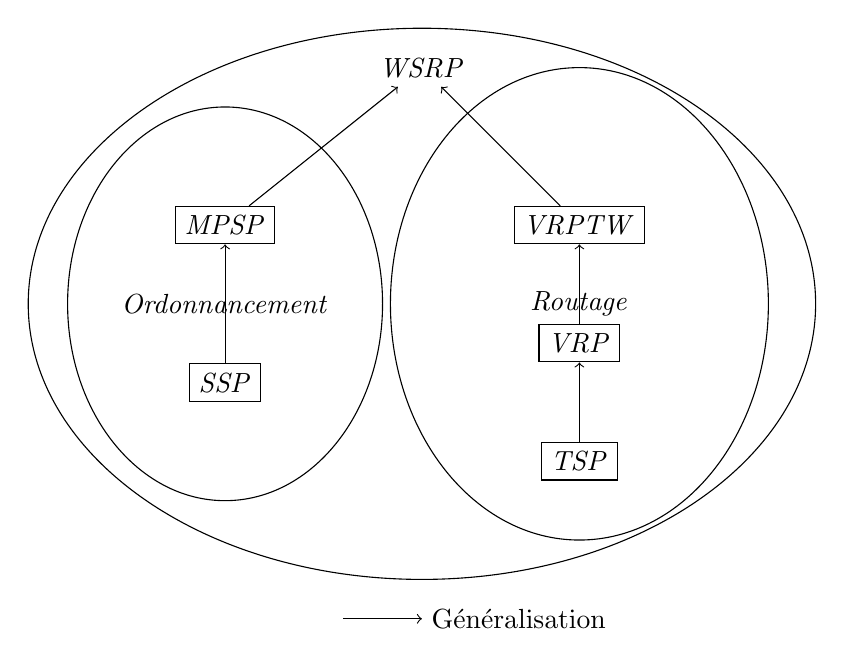
\begin{tikzpicture}
\node[] (0) at (0,0) {\textit{WSRP}};
\draw (0,-3) circle(5 and 3.5);
\draw (2,-3) circle(2.4 and 3) node[]{\textit{Routage}};
\draw (-2.5,-3) circle(2 and 2.5) node[]{\textit{Ordonnancement}};
\node[draw,rectangle] (4) at (-2.5,-4) {\textit{SSP}};

\node[draw,rectangle] (5) at (2,-3.5) {\textit{VRP}};
\node[draw,rectangle] (9) at (2,-5) {\textit{TSP}};

\draw[->] (9)--(5);

\node[draw,rectangle] (1) at (-2.5,-2) {\textit{MPSP}};
\node[draw,rectangle] (2) at (2,-2) {\textit{VRPTW}};
\draw[->] (4)--(1);
\draw[->] (5)--(2);

\draw[->] (2)--(0);
\draw[->] (1)--(0);
\draw[->] (-1,-7)--(0,-7) node[right] {Généralisation};
\end{tikzpicture}
\caption{Schéma représentant la classe de complexité de la classe WSRP \label{fig:complex:gloabale}}
\end{figure}


La figure~\ref{fig:complex:gloabale} représente les généralisations successives des problèmes d'ordonnancement et de routage de base, comme le \tsp, qui mènent à la classe de problèmes \wsrp.
Lorsque l'on dit qu'un problème $\pi_1$ est une généralisation d'un autre $\pi_2$ (ou alors que $\pi_2$ généralise $\pi_1$) cela veut dire qu'il est plus dur au sens de la complexité. 
Si on passe des instances de $\pi_2$ à $\pi_1$ alors ces instances n'utilisent qu'un sous-ensemble des contraintes de $\pi_1$.
Autrement dit, on peut modéliser des instances plus complexes en utilisant $\pi_1$ qu'en utilisant $\pi_2$.


\begin{comment}

\begin{figure}[H]

\centering
\begin{tikzpicture}

\node[draw,rectangle] (0) at (0,0) {\wsrp};

\node[draw,rectangle] (1) at (-2,-2) {\mpsp};
\node[draw,rectangle] (2) at (0,-2) {\vrptw};
\node[draw,rectangle] (3) at (2.5,-2) {\pdptw};

\node[draw,rectangle] (4) at (-2,-4) {\ssp};
\node[draw,rectangle] (5) at (0,-4) {\vrp};
\node[draw,rectangle] (6) at (2.5,-3) {\pdp};

\node[draw,rectangle] (7) at (-2.7,-6) {\rcpsp};
\node[draw,rectangle] (8) at (-1.2,-6) {$\ldots$};
\node[draw,rectangle] (9) at (0,-6) {\tsp};

\draw[->] (1)--(0);
\draw[->] (2)--(0);
\draw[->] (3)--(0);

\draw[->] (4)--(1);
\draw[->] (5)--(6);
\draw[->] (5)--(2);
\draw[->] (6)--(3);

\draw[->] (7)--(4);
\draw[->] (8)--(4);
\draw[->] (9)--(5);
%%%%%%%%%%%%% Légendes %%%%%%%%%%%%%%
\draw[->] (3.5,-5)--(4,-5);
\node[] at (3,-5) {A};
\node[] at (4.5,-5) {B};
\node[] at (3.75,-5.5) {$=$};
\node[] at (3.75,-6) {B généralise A};
\end{tikzpicture}

\caption{\label{Fig:Complexite} \'Evolution des problèmes : ajout de contraintes }
\end{figure}
\end{comment}

En ce qui concerne les méthodes de résolution, Rasmussen et al. \cite{Rasmussen2010} proposent une formulation MIP, et utilisent la génération de colonnes et une décomposition de Dantzig-Wolfe avec différentes méthodes de branchements dans l'algorithme de branch-and-price. Cependant avec leur méthode, ils ne résolvent pas à l'optimal des instances avec 15 employés, 150 tâches et environs 30\% de tâches avec des contraintes de précédences en moins de 20 minutes.

Xie et al. \cite{Xie2017} utilisent de la recherche locale itérée (iterated local search) pour résoudre des instances d'un problème de \wsrp.
Leur méthode est la suivante : ils construisent une solution réalisable, puis avec des opérateurs de voisinage (échange ou inversion de séquence) puis améliorent la solution jusqu'à potentiellement obtenir la solution optimale, cependant on perd la garantie d'optimalité et même de qualité de solution : on ne connaît pas l'écart entre la solution trouvée et la solution optimale.
Ils comparent leur méthode de résolution à une résolution exacte et à de l'ALNS sur des instances avec 30 techniciens et 100 tâches.
L'avantage de leur méthode est que la solution obtenue est de bonne qualité (gap de 1\%) et le vrai avantage est le temps d'exécution (moins d'une minute) alors que la recherche exacte (modèle MIP + cplex) utilisée met au plus 2 heures pour trouver la solution optimale.
